% !TEX TS-program = Xelatex
% !TEX encoding = UTF-8 Unicode

\documentclass[UTF8]{ctexart}
\usepackage{amsmath}
\usepackage[bottom]{footmisc}
\usepackage{geometry}
\usepackage{graphicx}
\usepackage{figsize}
\usepackage[separate-uncertainty = true,per-mode=symbol]{siunitx}
\usepackage{tabu}
\usepackage{wasysym}
\geometry{left=0.7in,right=0.7in,bottom=0.7in,top=0.7in}

\title{实验十五:非平衡电桥测Pt100的温度系数}
\author{朱寅杰 1600017721}
\date{2017年11月10日}

\begin{document}

\maketitle

\section{Pt100}
$R_p=\SI{100.2}{\ohm}$。恒流源电流为$I=\SI{4.006}{\milli\ampere}$。
\begin{center}
\begin{tabu} to \linewidth {X[c]|X[c] X[c] X[c] X[c] X[c] X[c] X[c]}
\hline
$t/\si{\celsius}$	&0.1	&21.2	&44.4	&56.8	&71.5	&85.6	&100.1
\\
\hline
$U/\si{\milli\volt}$	&0.00	&16.02	&33.80	&43.32	&54.37	&65.05	&76.07
\\
\hline
\end{tabu}
\end{center}

\begin{figure}[h]
  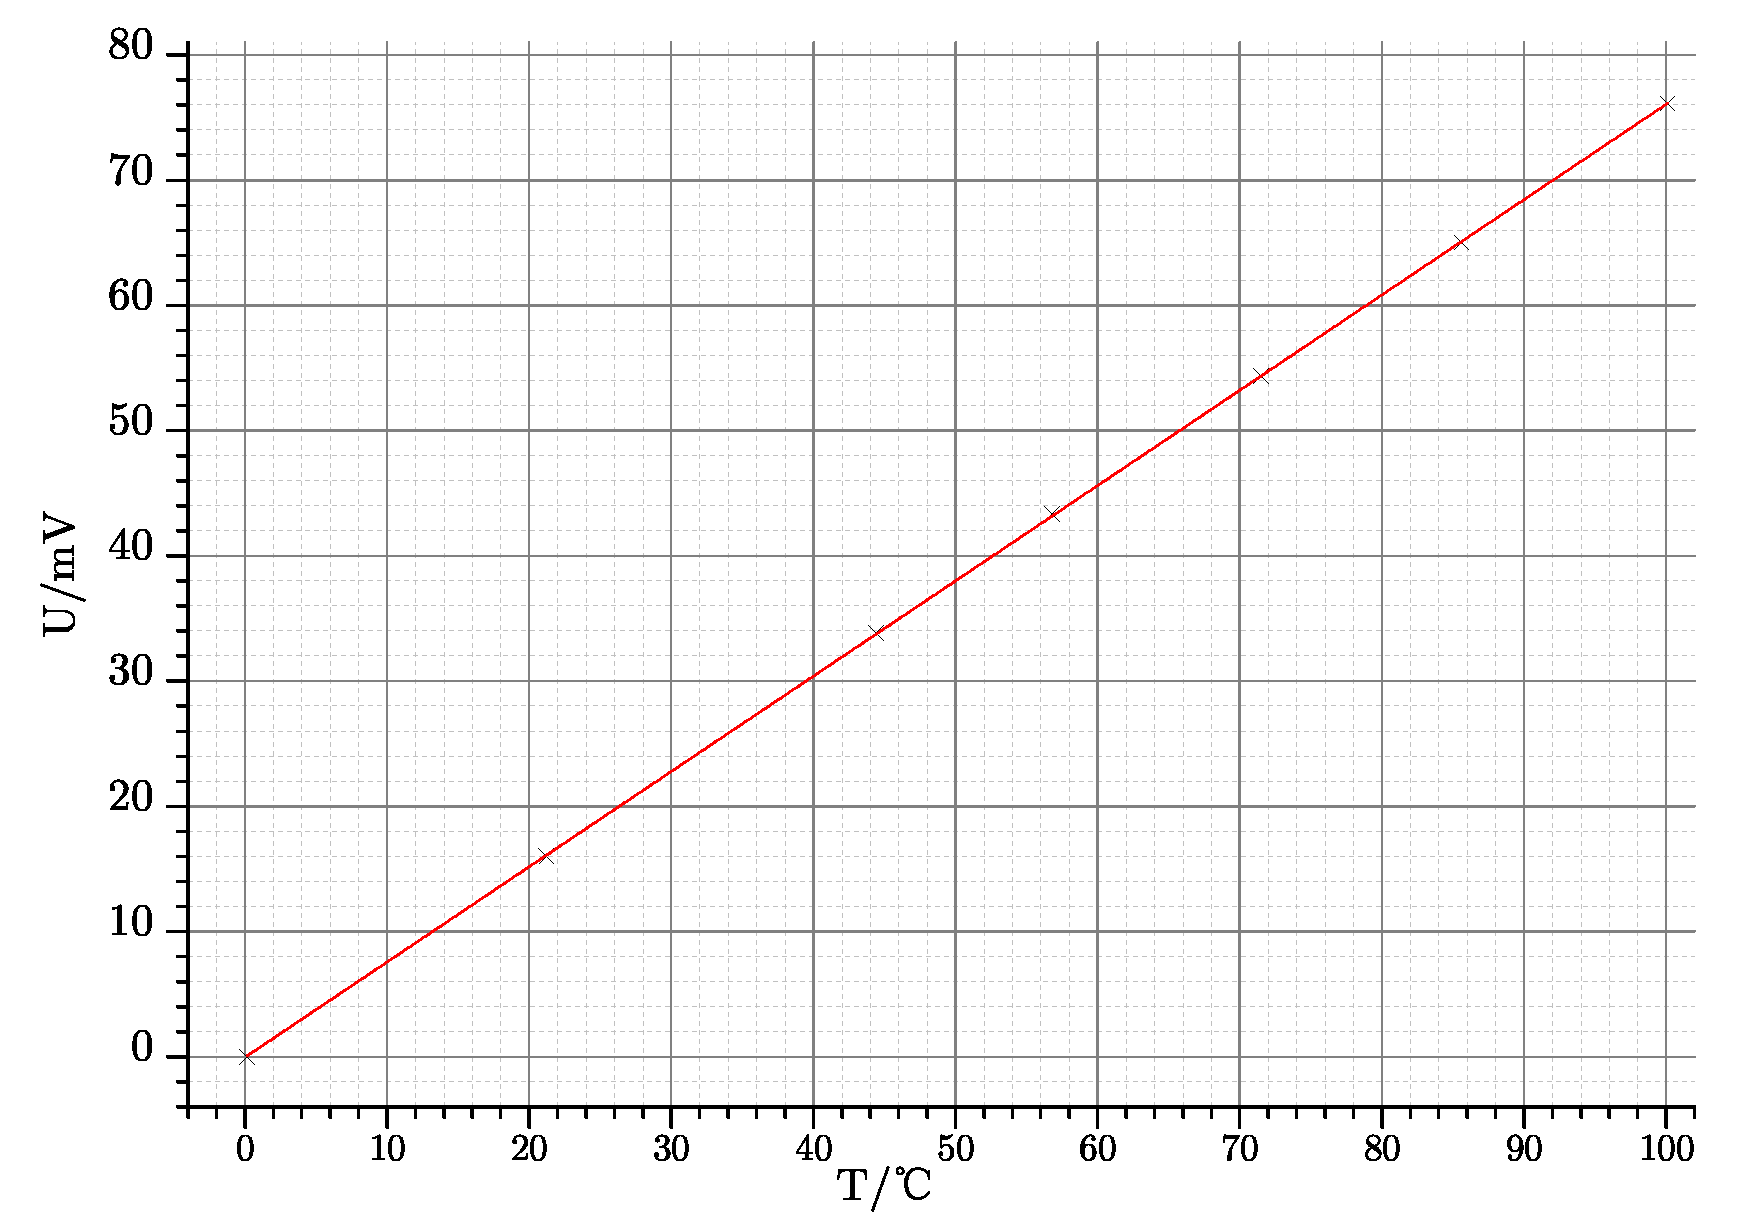
\includegraphics[width=\linewidth,keepaspectratio=true]{Pt100.eps}
  \caption{$U-t$关系图。}
\end{figure}
对表中数据作线性拟合得到
\begin{equation}
  U=\SI{.04}{\milli\volt}+\SI{.7609}{\milli\volt\per\celsius}\times t
\end{equation}
$r=\num{.999996}$
因此斜率的不确定度有
\section{思考题}
%见王彬旭的实验报告
\end{document}